\chapter{电解与极化作用}

\begin{itemize}
    \item 可逆电极:平衡,$I \to 0$,无限时间,$\phi_{\mbox{可逆}}$
    \item 不可逆电极:不平衡,$I \neq 0$,不可逆的电极过程,有限时间,$\phi_{\mbox{不可可逆}}$
\end{itemize}


本章主要研究:不可逆电极的电极作用、电解时的真正的充放电效应。



\section{分解电压}

分解电压,指使电解质在电极上分解生成电解产物所需施加的最小电压。电解质的分解电压由其电解产物组成的元电池电动势,阴阳二电极的极化过电位和电路压降三部分组成。

\begin{align*}
    E_{\mbox{分解}} &= E_{\mbox{可逆}} \\ 
    E_{\mbox{分解}} &= E_{\mbox{不可逆}} + \Delta E + IR \\ 
\end{align*}


\section{极化作用}


不可逆电极过程中$\phi$偏离平衡位置的现象。

产生极化的原因:当$I \neq 0$时,电极上发生一系列以一定速率进行的过程。每个过程均有阻力,克服阻力需要推动力,就表现为$\phi$的偏离行为。电池极化分为:

\subsection{浓差极化}

由于浓差扩散过程中存在阻力,使得电极附近的溶液与浓度的本体不同,从而使$\phi$值与平衡值产生一定的偏离。

\subsection{电化学极化}


电极反应的某一步反应速率比较慢,需要比较高的活化能。


\section{超电势}


某一电流密度下,实际发生电解的电极电势$\phi$和可逆电极$\phi_0$之间的差距称为超电势。

\subsection{极化曲线}


在给定电流$i$下,电池或电解池中阴极和阳极的实际电极电势的值称为极化曲线。总体上看由于极化的存在不利于能量的利用。

\begin{figure}[h]
    \centering
    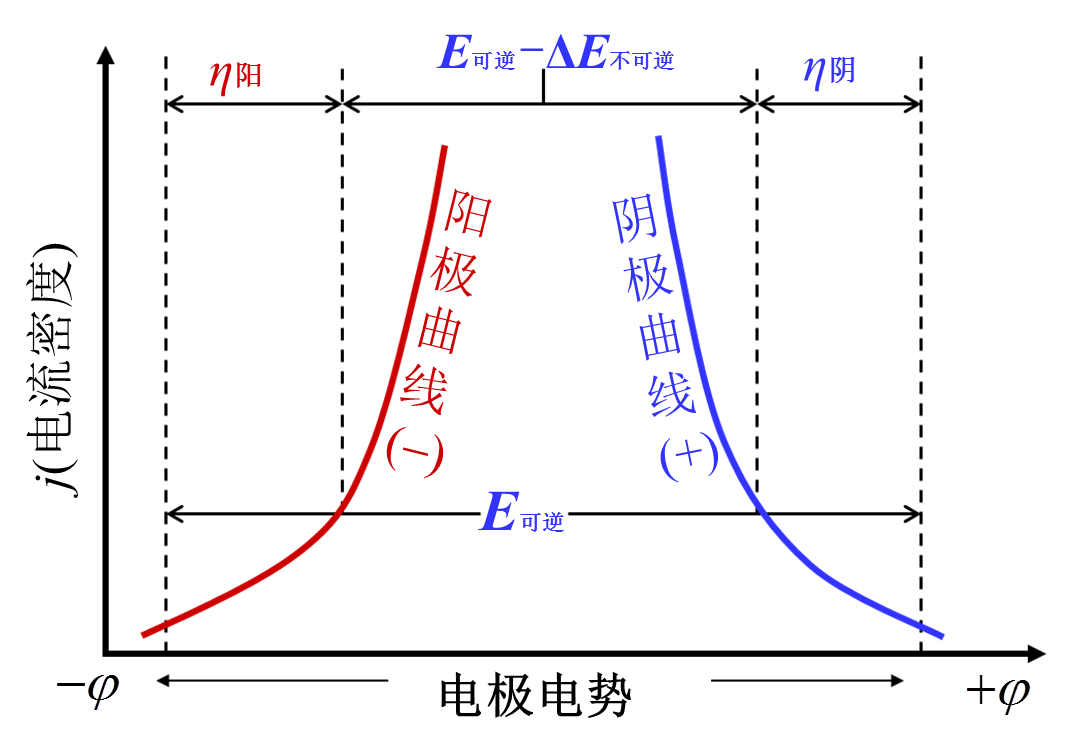
\includegraphics[width=0.7\textwidth]{battery_dmii.png}
    \caption{电池的极化曲线}
    \label{fig:battery_dmii}
\end{figure}

\begin{figure}[h]
    \centering
    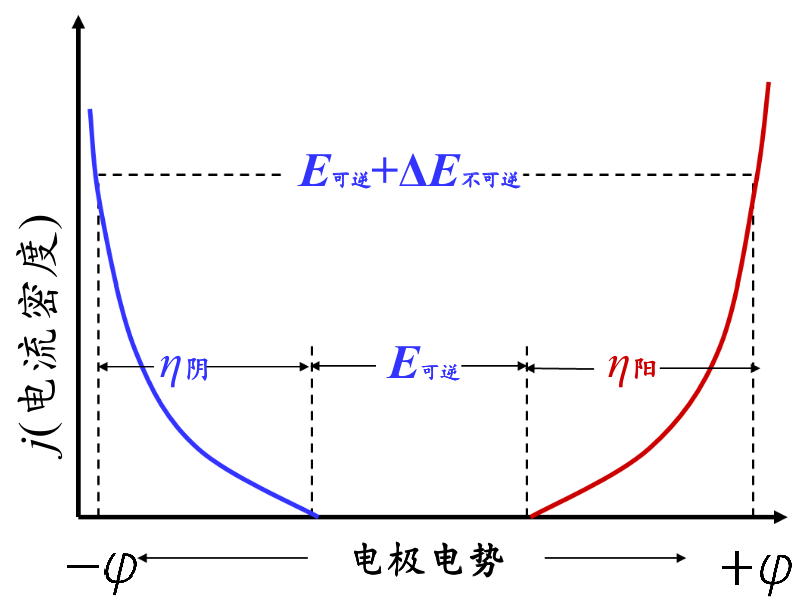
\includegraphics[width=0.7\textwidth]{cell_dmjpii.png}
    \caption{电解池的极化曲线}
    \label{fig:cell_dmjpii}
\end{figure}
